\documentclass[eng,printmode,openany]{mgr}
\usepackage[utf8]{inputenc}
\usepackage{polski}
\usepackage[polish]{babel}
\usepackage{graphicx}
\usepackage{subfigure}

\usepackage{psfrag}
\usepackage{amsmath}
\usepackage{amsfonts}

\usepackage{supertabular}
\usepackage{array}
\usepackage{tabularx}
\usepackage{hhline}
\usepackage{showlabels}
\usepackage{float}
\usepackage[square,sort,comma,numbers]{natbib}


\newcommand{\R}{I\!\!R}
\newtheorem{theorem}{Twierdzenie}[section]

% frontpage
\title{Aplikacja webowa wspomagająca zarządzanie flotą samochodów}
\engtitle{A web application supporting cars fleet management}
\author{Jan Pajdak}
\supervisor{dr inż. Jarosław Mierzwa, K-9}
\guardian{dr hab. inż. Olgierd Unold Prof. nadzw. PWr, K-9}
\field{Informatyka (INF)}
\specialisation{Inżynieria systemów informatycznych (INS)}

\begin{document}
%\bibliographystyle{plabbrv}
\bibliographystyle{plainnat} 

\maketitle
%\dedication{6cm}{dedykacja \texttt{$\backslash$dedication}}

\tableofcontents 

%----------------------------------------------------------------------------------------
%	SECTION 0
%----------------------------------------------------------------------------------------

%----------------------------------------------------------------------------------------
%	SECTION 1
%----------------------------------------------------------------------------------------
% cel, zakres pracy
\chapter{Wprowadzenie}
\section{Wstęp}
Celem niniejszej pracy dyplomowej jest opracowanie projektu, implementacja oraz wdrożenie systemu umożliwiającego zarządzanie flotą samochodów. Pierwszym etapem projektu jest zebrane wymagań funkcjonalnych i niefunkcjonalnych oraz określenie zakresu pracy. Drugi etap projektu to wybór technologii i projekt architektury. Ostatnim celem jest implementacja systemu.

Temat projektu został wybrany ze względu na chęć wykorzystania wiedzy z dziedziny motoryzacji w celu stworzenia aplikacji ułatwiającej zarządzanie pojazdami. Z uwagi na rosnącą popularność rozwiązań związanych z wypożyczaniem samochodów celem projektu jest system, który można opisać jako wewnątrzfirmową wypożyczalnie umożliwiająca jak największe wykorzystanie dostępnej floty pojazdów przez pracowników, którzy nie mają potrzeby posiadania firmowego samochodu na wyłączność. 

\section{Cel i zakres pracy}
Celem projektu jest stworzenie aplikacji umożliwiającej wypożyczanie oraz zarządzanie flotą samochodów. Aplikacja jest skierowana do firm które nie mają potrzeby lub wystarczających środków by zapewnić pracownikom samochody na wyłączność. Przykładowym przypadkiem użycia systemu może być jednorazowa potrzeba odwiedzenia klienta lub wyjazd na szkolenie. Typowe rozwiązania dla firm obecne na rynku skierowane są do firm świadczących usługi spedycyjne — aplikacje posiadają warstwę śledzenia ładunków oraz tworzenia zadań przewozowych dla kierowców; programy służące do obsługi komercyjnych wypożyczalni pomijają proces autoryzacji wypożyczenia — zwykle sprawdzana jest zdolność wypożyczającego do zapłaty.

Projekt utworzony w ramach tej pracy łączy mechanikę z komercyjnych wypożyczalni z dodatkową warstwą biznesową pozwalającą kontrolować sposób używania pojazdów.

Zakres pracy obejmuje utworzenie systemu spełniającego wymagania postawione w rozdziale 3 oraz przygotowanie projektu do wdrożenia, poprzez np. konteneryzacje.

\section{Układ pracy}
W rozdziale pierwszym zawarto wstęp oraz krótki opis celu projektu. Drugi rozdział porównuje istniejące rozwiązania do aplikacji będącej celem projektu. Rozdział trzeci zawiera wymagania funkcjonalne oraz niefunkcjonalne. W kolejnym, czwartym rozdziale znajduje się opis wybranych technologii oraz narzędzi, wraz z uzasadnieniem. 

%----------------------------------------------------------------------------------------
%	SECTION 2
%----------------------------------------------------------------------------------------
\newpage
\chapter{Istniejące rozwiązania}

%----------------------------------------------------------------------------------------
%	SECTION 3
%----------------------------------------------------------------------------------------
\newpage
\chapter{Wymagania funkcjonalne i niefunkcjonalne}
\section{Wymagania funkcjonalne}
Wymagania zostały opisane według poniższego wzorca:
%	\item Aktor - grupa użytkowników systemu; rozróżniane są dwa rodzaje aktorów:
%	\subitem Kierowca - użytkownik mający dostęp wyłącznie to tworzenia wypożyczeń
%	\subitem Kierownik - użytkownik z pełnym dostępem do systemu 
\begin{table}[H]
	\begin{tabularx}{\textwidth}{|l|X|}
		\hline
		Numer                & Numer wymagania \\ \hline
		Nazwa                & Krótka nazwa\\ \hline
		Opis                 & Dokładny opis\\ \hline
		Aktor                & Grupa użytkowników\\ \hline
		Kryterium spełnienia & Funkcjonalność która musi zostać zaimplementowana by wymaganie można było uznać jako spełnione\\ \hline
		Ograniczenia         & Ograniczenia funkcjonalności, jeżeli takie istnieją\\ \hline
	\end{tabularx}
\end{table}
Rozróżniane są dwa rodzaje aktorów:
\begin{itemize}
	\item Kierowca - użytkownik korzystający z funkcjonalności tworzenia i przeglądania historii wypożyczeń
	\item Kierownik - użytkownik z pełnym dostępem do systemu
\end{itemize}
Kierownik posiada wszelkie prawa i możliwości Kierowcy.

Dodatkowe pojęcia związane z modelami świata biznesowego:
\begin{itemize}
	\item \textbf{Model Pojazdu} - model opisujący specyfikacje techniczną wspólną dla pewnego zbioru pojazdów
	\item \textbf{Pojazd} - model opisujący informacje unikatowe dla pewnego przedstawiciela zbioru Modeli Pojazdów.
\end{itemize}

\begin{table}[H]
	\begin{tabularx}{\textwidth}{|l|X|}
		\hline
		Numer                & 1  \\ \hline
		Nazwa                & Zarządzanie modelami pojazdów \\ \hline
		Opis                 & System powinien pozwalać na dodawanie i edycję modeli pojazdów; specyfikacji technicznej dla danego modelu.    \\ \hline
		Aktor                & Kierownik \\ \hline
		Kryterium spełnienia & Kierownik może dodawać nowe modele samochodów. Informacje mogą zostać w późniejszym czasie zmodyfikowane lub usunięte.\\ \hline
		Ograniczenia         & Model pojazdu może zostać usunięty wyłącznie gdy nie ma żadnych pojazdów \\ \hline
	\end{tabularx}
\end{table}

\begin{table}[H]
	\begin{tabularx}{\textwidth}{|l|X|}
		\hline
		Numer                & 2 \\ \hline
		Nazwa                & Zarządzanie pojazdami \\ \hline
		Opis                 & System powinien pozwalać na dodawanie i edycję pojazdów będących egzemplarzami modeli z wymagania \#2; pojazd zawiera informacje unikalne dla danego egzemplarza, takie jak numer rejestracyjny.     \\ \hline
		Aktor                & Kierownik \\ \hline
		Kryterium spełnienia & Kierownik może dodawać nowe pojazdy dla wybranego modelu. Informacje mogą zostać w późniejszym czasie zmodyfikowane lub usunięte.\\ \hline
		Ograniczenia         & Pojazd nie może być modyfikowany gdy jest obecnie wypożyczony. Pojazd który był wypożyczany nie może zostać usunięty — może zostać oznaczony jako wycofany z użycia. \\ \hline
	\end{tabularx}
\end{table}

\begin{table}[H]
	\begin{tabularx}{\textwidth}{|l|X|}
		\hline
		Numer                & 3 \\ \hline
		Nazwa                & Zarządzanie ubezpieczeniami pojazdu \\ \hline
		Opis                 & System powinien umożliwiać wprowadzanie informacji związanych z ubezpieczeniami danego pojazdu. \\ \hline
		Aktor                & Kierownik \\ \hline
		Kryterium spełnienia & Kierownik może przeglądać historię ubezpieczeń danego pojazdu oraz wprowadzać nowe dane. System bierze pod uwagę obecny stan pojazdu podczas tworzenia wypożyczenia;  pojazd nie może zostać wypożyczony w okresie gdy nie ma aktywnego ubezpieczenia. \\ \hline
		Ograniczenia         & \\ \hline
	\end{tabularx}
\end{table}

\begin{table}[H]
	\begin{tabularx}{\textwidth}{|l|X|}
		\hline
		Numer                & 4 \\ \hline
		Nazwa                & Zarządzanie serwisami pojazdu \\ \hline
		Opis                 & System powinien umożliwiać wprowadzanie informacji związanych z serwisami danego pojazdu. \\ \hline
		Aktor                & Kierownik \\ \hline
		Kryterium spełnienia & Kierownik może przeglądać historię napraw danego pojazdu oraz wprowadzać nowe dane. System rozróżnia różne rodzaje serwisowania takie jak regularny przegląd, zdarzenie wyjątkowe czy naprawa powypadkowa. System bierze pod uwagę obecny stan pojazdu podczas tworzenia wypożyczenia; pojazd nie może zostać wypożyczony gdy jest obecnie naprawiany. \\ \hline
		Ograniczenia         & \\ \hline
	\end{tabularx}
\end{table}

\begin{table}[H]
	\begin{tabularx}{\textwidth}{|l|X|}
		\hline
		Numer                & 5 \\ \hline
		Nazwa                & Tworzenie wypożyczeń \\ \hline
		Opis                 & System powinien umożliwiać przeglądanie dostępnych pojazdów (dostępność określana jest na podstawie informacji z wymagania \#2) i tworzenie wypożyczeń wraz z niezbędnymi danymi takimi jak okres czasu i potrzeba stojąca za wypożyczeniem\\ \hline
		Aktor                & Kierowca \\ \hline
		Kryterium spełnienia & Kierowca może utworzyć wypożyczenie \\ \hline
		Ograniczenia         & Kierowca nie może utworzyć wypożyczenia dla innego użytkownika \\ \hline
	\end{tabularx}
\end{table}

\begin{table}[H]
	\begin{tabularx}{\textwidth}{|l|X|}
		\hline
		Numer                & 6 \\ \hline
		Nazwa                & Kontrola wypożyczeń\\ \hline
		Opis                 & System umożliwia kontrolowanie stanu wypożyczenia. Wypożyczenie uznane jest za obowiązujące dopiero po akceptacji przez uprawnioną do tego osobę.\\ \hline
		Aktor                & Kierownik \\ \hline
		Kryterium spełnienia & Kierownik może przeglądać wypożyczenia utworzone przez użytkowników systemu oraz zmieniać ich obecny stan po ocenie zasadności wypożyczenia \\ \hline
		Ograniczenia         & Kierownik nie może akceptować własnych wypożyczeń \\ \hline
	\end{tabularx}
\end{table}

\begin{table}[H]
	\begin{tabularx}{\textwidth}{|l|X|}
		\hline
		Numer                & 7 \\ \hline
		Nazwa                & Zbieranie informacji o kosztach wypożyczeń\\ \hline
		Opis                 & System umożliwia śledzenie kosztów utrzymania floty na podstawie raportów wprowadzanych przez wypożyczających. \\ \hline
		Aktor                & Kierowca\\ \hline
		Kryterium spełnienia & Kierowca może wprowadzić informację związane z wypożyczeniem (zużyte litry paliwa, przejechane kilometry, całkowity koszt) po oddaniu samochodu.\\ \hline
		Ograniczenia         & \\ \hline
	\end{tabularx}
\end{table}

\begin{table}[H]
	\begin{tabularx}{\textwidth}{|l|X|}
		\hline
		Numer                & 8 \\ \hline
		Nazwa                & Zbieranie informacji o kosztach utrzymania \\ \hline
		Opis                 & System umożliwia śledzenie kosztów utrzymania floty związanych z ubezpieczeniami oraz naprawami. \\ \hline
		Aktor                & Kierownik \\ \hline
		Kryterium spełnienia & Kierownik może wprowadzić koszty związane z ubezpieczeniem/serwisem pojazdu. \\ \hline
		Ograniczenia         & \\ \hline
	\end{tabularx}
\end{table}

\begin{table}[H]
	\begin{tabularx}{\textwidth}{|l|X|}
		\hline
		Numer                & 9 \\ \hline
		Nazwa                & Wyświetlanie informacji o kosztach utrzymania \\ \hline
		Opis                 & System jest w stanie wygenerować plik kompatybilny z programem \textit{Excel} zawierający dane na temat kosztów floty. \\ \hline
		Aktor                & Kierownik \\ \hline
		Kryterium spełnienia & Kierownik może wywołać utworzenie pliku ze statystykami  \\ \hline
		Ograniczenia         & \\ \hline
	\end{tabularx}
\end{table}

\begin{table}[H]
	\begin{tabularx}{\textwidth}{|l|X|}
		\hline
		Numer                & 10 \\ \hline
		Nazwa                & Przechowywanie informacji audytowych \\ \hline
		Opis                 & System zapisuje informacje o dacie i użytkowniku dokonującym wprowadzenia nowych danych lub modyfikacji istniejących. \\ \hline
		Aktor                & Kierownik \\ \hline
		Kryterium spełnienia & Informacje o dacie i użytkowniku modyfikowane są w trakcie zapisu do bazy danych. Kierownik może przeglądać dane audytowe.  \\ \hline
		Ograniczenia         & \\ \hline
	\end{tabularx}
\end{table}

\section{Wymagania niefunkcjonalne}
\subsection{Interfejs użytkownika}
\begin{itemize}
	\item Wygląd powinien być prosty i nowoczesny
	\item Elementy strony powinny być rozmieszczone w intuicyjny sposób
	\item Struktura widoków powinna być ułożona zgodnie z zależnościami między wyświetlanymi danymi
	\item Aplikacja być wygodna w użyciu na ekranach komputerów o rozdzielczości HD (1366x768 pikseli) lub większej
\end{itemize}
\subsection{Interfejs programistyczny}
\begin{itemize}
	\item System powinien wymagać niewielkich modyfikacji w przypadku integracji z istniejącymi zasobami firmy (np. baza danych pracowników)
	\item Komunikacja powinna opierać się na otwartych i uniwersalnych standardach, np. dane w postaci \textit{JSON} lub \textit{XML} przesyłane protokołem \textit{HTTP}
	\item Interfejs programistyczny powinien być niezależny od platformy tak by w przyszłości mógł zostać wykorzystany przez inne aplikacje
\end{itemize}
\subsection{Bezpieczeństwo}
System powinien być zabezpieczony zarówno po stronie interfejsu użytkownika (np. blokada przed przejściem do podstrony) oraz po stronie interfejsu programistycznego (ignorowanie zapytań od nieupoważnionych aplikacji). Zabezpieczenie powinno obsługiwać różne poziomy autoryzacji w zależności od roli użytkownika.

%----------------------------------------------------------------------------------------
%	SECTION 4
%----------------------------------------------------------------------------------------
\newpage
\chapter{Zastosowane technologie i narzędzia}
\section{Zastosowane technologie}
Interfejs użytkownika wykorzystuje platformę \textit{Angular 7}. Podstawowymi elementami w \textit{Angular} są komponenty \cite{angular-components}, każdy z nich złożony z: pliku klasy \textit{TypeScript} zawierającej logikę, wzorca \textit{htm} opisującego wygląd widoku oraz opcjonalnego stylu \textit{css}; w przypadku jego braku styl brany jest z komponentu-rodzica. Warto zwrócić uwagę na język programowania wykorzystywany przez platformę \textit{Angular} — \textit{TypeScript} \cite{msdn-ts}, będący rozszerzeniem języka \textit{JavaScript}. \textit{TypeScript} dodaje silniejsze typowanie i kładzie większy nacisk na programowanie obiektowe, jednocześnie pozostając w pełni kompatybilnym z \textit{JavaScript}, do którego jest kompilowany i  następnie uruchamiany jest w przeglądarce. Proces kompilacji pozwala na usunięcie wielu błędów, które w przypadku \textit{JavaScript} zostałyby zauważone dopiero po uruchomieniu aplikacji.

Jednym z ważniejszych komponentów aplikacji jest \textit{Bootstrap} - framework interfejsu użytkownika pozwalający w prosty sposób tworzyć estetyczne strony internetowe. Dodatkowo, w projekcie wykorzystano motywy \textit{Bootswatch}.

Interfejs programistyczny oparty został na technologii \textit{ASP.NET Core 2.1} — jest to nowoczesna platforma oferująca działanie na wielu systemach operacyjnych oraz większa wydajność względem starszych rozwiązań firmy Microsoft. Wykorzystany język programowania to obiektowy, kompilowany i statycznie typowany \textit{C\# 7.3}. Bardzo ważnym elementem tej części projektu jest \textit{EF (Entity Framework) Core 2.1} \cite{msdn-efcore}, framework ORM (Object-Relational Mapping) pozwalający na konwersję miedzy tabelami bazy danych a klasami \textit{C\#}. Jedną z najważniejszych funkcjonalności \textit{EF Core} jest wykorzystana w niniejszym projekcie możliwość utworzenia bazy danych przy użyciu konwencji \textit{Code First}; baza danych jest automatycznie generowana na podstawie klas \text{C\#} znajdujących się w projekcie. \textit{EF Core} współpracuje z większością popularnych baz danych; na potrzeby tego projektu wykorzystano \textit{MS SQL Server}.

\section{Wykorzystane narzędzia}
W trakcie realizacji projektu wykorzystane zostały narzędzia najczęściej używane przy wybranych technologiach.

Do zarządzania kodem został wykorzystany system kontroli wersji \textit{Git}. Lokalna kopia projektu była synchronizowana ze zdalnym, prywatnym repozytorium znajdującym się na serwisie \text{GitHub}. Wykorzystane rozwiązanie pozwala na łatwy dostęp do wcześniejszych wersji projektu oraz zmniejsza ryzyko utraty kodu, gdyż nie jest on przechowywany tylko w jednym miejscu.

Ze względu na wykorzystane technologie, kod był rozwijany z pomocą narzędzi Microsoft, oferujących najlepsze wsparcie dla \textit{TypeScript} oraz \textit{C\#}. Aplikacja klienta była rozwijana przy użyciu \textit{Visual Studio Code 1.28}, nowoczesnego edytora który sprawdza się znakomicie przy tworzeniu interfejsów użytkownika ze względu na zintegrowaną konsolę pozwalającą na łatwe zarządzanie paczkami oraz łatwość dostosowywania do potrzeb użytkownika. W trakcie pracy wykorzystano wiele rozszerzeń, najważniejsze z nich to \textit{TSLint}, linter wykrywający błędy w kodzie \textit{TypeScript} oraz \textit{GitLens} — rozszerzenie wspomagające zarządzanie repozytorium \textit{Git}. Do rozwoju serwisów wykorzystano \textit{Visual Studio 2017} pozwalające na łatwe debugowanie kodu oraz analizę aspektów takich jak wykorzystanie zasobów przez program. \textit{Visual Studio} zostało wzbogacone o narzędzie \textit{JetBrains ReSharper} automatycznie formatujące pliki projektu według zadanego wzorca, zapewniając spójność i przejrzystość kodu.

Interfejs programistyczny testowany był przy pomocy \textit{Postman 6.5.2}, aplikacji pozwalającej na wysyłanie oraz zarządzanie zapytaniami HTTP.

%----------------------------------------------------------------------------------------
%	SECTION 5
%----------------------------------------------------------------------------------------
\newpage
\chapter{Projekt}
\section{Architektura}
System został stworzony przy użyciu klasycznej architektury w której można wyodrębić trzy moduły - interfejs użytkownika (\textit{UI}), interfejs programistyczny (\textit{API}) oraz bazę danych (\textit{DB}). 

\begin{figure}[h]
	\centering
	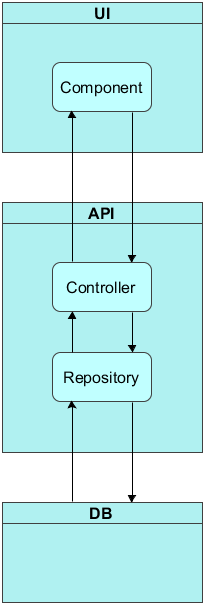
\includegraphics[scale=0.6]{images/architecture.png}
	\caption{Uproszczony schemat architektury z wyodrębnionymi najważniejszymi elementami składowymi}
\end{figure}


System został zaprojektowany tak, by mógł zostać zintegrowany z istniejącymi zasobami firmy — jedyne dane, jakie przechowuje, dotyczą logiki biznesowej, związanej z wymaganiami funkcjonalnymi; wynika to z faktu, że większość firm ma już własne bazy danych przechowujące informacje o pracownikach więc duplikacja danych jest niepożądana ze względu na zużycie zasobów oraz możliwe problemy z synchronizacją. Dane związane z użytkownikami (np. imię, nazwisko, e-mail i numer telefonu) czy lokacjami firmy (np. adres) mogą zostać pobrane z innej bazy danych; ponadto interfejs użytkownika nie umożliwia wprowadzania lub edycji takich danych. Implementacja opisana w dalszej części niniejszej pracy przechowuje przykładowe dane użytkowników do celów testowych w tej samej bazie danych, jednakże konfiguracja systemu tak by korzystał z innej, nie stanowi większego problemu.

W architekturze można rozróżnić trzy najważniejsze składowe, dwie pierwsze w interfejsie programistycznym i trzecią w interfejsie użytkownika:
\begin{itemize}
	\item Kontroler (\textit{Controller}) to klasa odpowiadająca za obsługę żądań \textit{HTTP} \cite{msdn-aspnet-api}.
	\item Repozytorium (\textit{Repository}) zawiera logikę pośredniczącą w komunikacji między \textit{API} a bazą danych.
	\item Komponent (\textit{Component}) to podstawowy element definiujący działanie widoku w \textit{Angular} \cite{angular-components}.
\end{itemize}

\section{Standardy}
Projekt był tworzony zgodnie z dobrymi praktykami programowania, z naciskiem na poprawną implementację obiektowego paradygmatu programowania. Interfejs programistyczny był tworzony z użyciem sztandarowych możliwości języka C\# takimi jak typy ogólne \cite{msdn-generics} (\textit{Generics}) pozwalające na tworzenie pojedynczych metod i klas zdolnych do operacji na wielu typach, zachowując wszystkie zalety silnego, statycznego typowania i wysoką wydajność.

W celu zapewnienia przejrzystości kodu, nazewnictwo wszystkich elementów oraz dokumentacja kodu są zgodne ze standardową konwencją danego języka. Kod jest napisany w całości w języku angielskim.
\begin{table}[H]
	\begin{tabularx}{\textwidth}{|l|l|l|l|l|}
		\hline
		Język      & Typy       			& Pliki                 & Zmienne prywatne & Inne zmienne \\ \hline
		C\# \cite{msdn-gnc}     & PascalCase & PascalCase.cs   		& camelCase        & PascalCase   \\ \hline
		TypeScript \cite{angular-sg} & PascalCase & snake-case.typ.ts 	& camelCase        & camelCase    \\ \hline
	\end{tabularx}
	\caption{Najważniejsze konwencje nazewnicze}
\end{table}

\section{Układ interfejsu użytkownika}
Komponenty (widoki) wchodzące w skład interfejsu użytkownika można podzielić na dwa główne rodzaje:
\begin{itemize}
	\item \textbf{Widok szczegółowy} (\textit{detail}) który zawiera komplet informacji o danym obiekcie i umożliwia jego edycję.
	\item \textbf{Widok listy} (\textit{list}) zawierający małą ilość informacji wymaganych do identyfikacji danego obiektu oraz możliwość przejścia do \textbf{widoku szczegółowego}. Widoki tego typu są punktem wejściowym do bardziej zaawansowanej logiki interfejsu, dostępnym bezpośrednio za pomocą paska nawigacji (\textit{navbar}).
\end{itemize}
\begin{figure}[h]
	\centering
	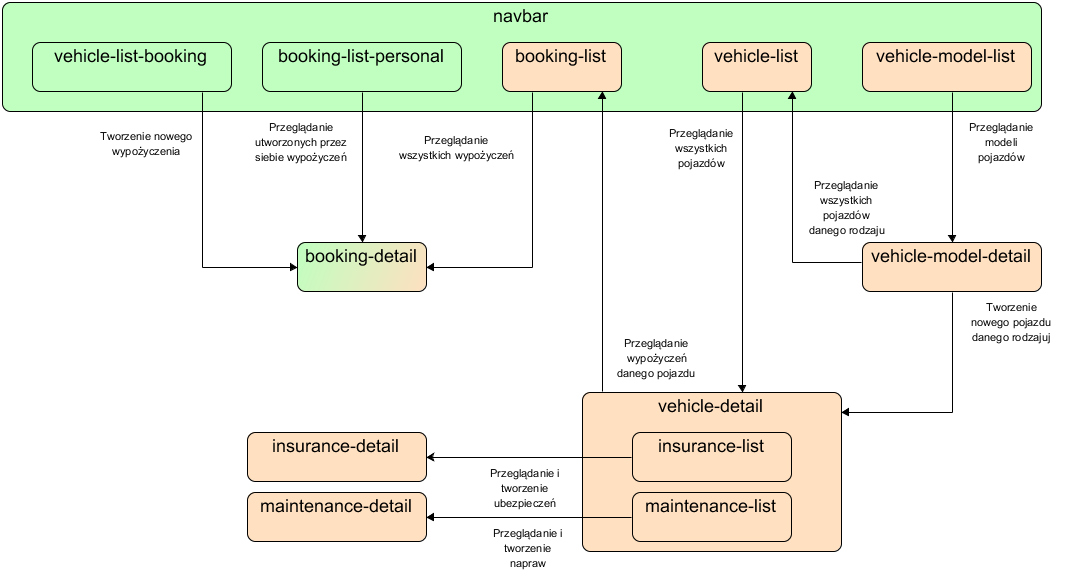
\includegraphics[scale=0.62]{images/angular_views.png}
	\caption{Widoki interfejsu użytkownika}
	\small 
	Widoki zielone dostępne są dla każdego użytkownika; widoki pomarańczowe wyłącznie dla użytkownika o odpowiednich uprawnieniach. Widok \textit{booking-detail} jest specjalnym przypadkiem oferującym różne możliwości w zależności od uprawnień użytkownika.
\end{figure}

\section{Bezpieczeństwo}
Dostęp do systemu został zabezpieczony przy użyciu standardu \textit{JSON Web Token (JWT)} \cite{jwt}. Autoryzacja \textit{JWT} bazuje na generowaniu podpisanych (przez co odpornych na sfałszowanie) tokenów po stronie interfejsu programistycznego, a następnie wysyłaniu ich do aplikacji klienta. \textit{API} wcześniej wygenerowanego wymaga tokena w nagłówku \textit{HTTP} dla każdego żądania wysłanego przez interfejs użytkownika; żądania z niepoprawnym tokenem zostają odrzucone.

Schemat działania autoryzacji \textit{JWT} w opisywanym projekcie wygląda następująco:
\begin{enumerate}
	\item Użytkownik loguje się przez interfejs użytkownika, podając nazwę użytkownika oraz hasło
	\item Interfejs programistyczny weryfikuje dane logowania
	\item W przypadku prawidłowego hasła utworzony zostaje token \textit{JWT} zawierający:
		\subitem Informacje o wydającym token
		\subitem Informacje o użytkowniku: jego identyfikator (nazwa użytkownika) oraz role
	\item Utworzony token zostaje zaszyfrowany (uniemożliwiając jego sfałszowanie) i zwrócony	
	\item Odebrany token zostaje umieszczony w pamięci przeglądarki internetowej użytkownika
\end{enumerate}
Interfejs programistyczny weryfikuje poprawność tokena dla każdego żądania \textit{HTTP} z wyjątkiem tych związanych z procesem autoryzacji użytkownika; jeżeli token jest niepoprawny lub zbyt stary (wydany więcej niż 2 godziny przed weryfikacją), żądanie jest odrzucone.

Przechowywanie ról w tokenie \textit{JWT} pozwala na autoryzację z uwzględnieniem uprawnień użytkownika, przykładowo, ograniczając dostęp do poufnych informacji lub modyfikacji przechowywanych danych przez osoby nieuprawnione.

\begin{figure}[h]
	\centering
	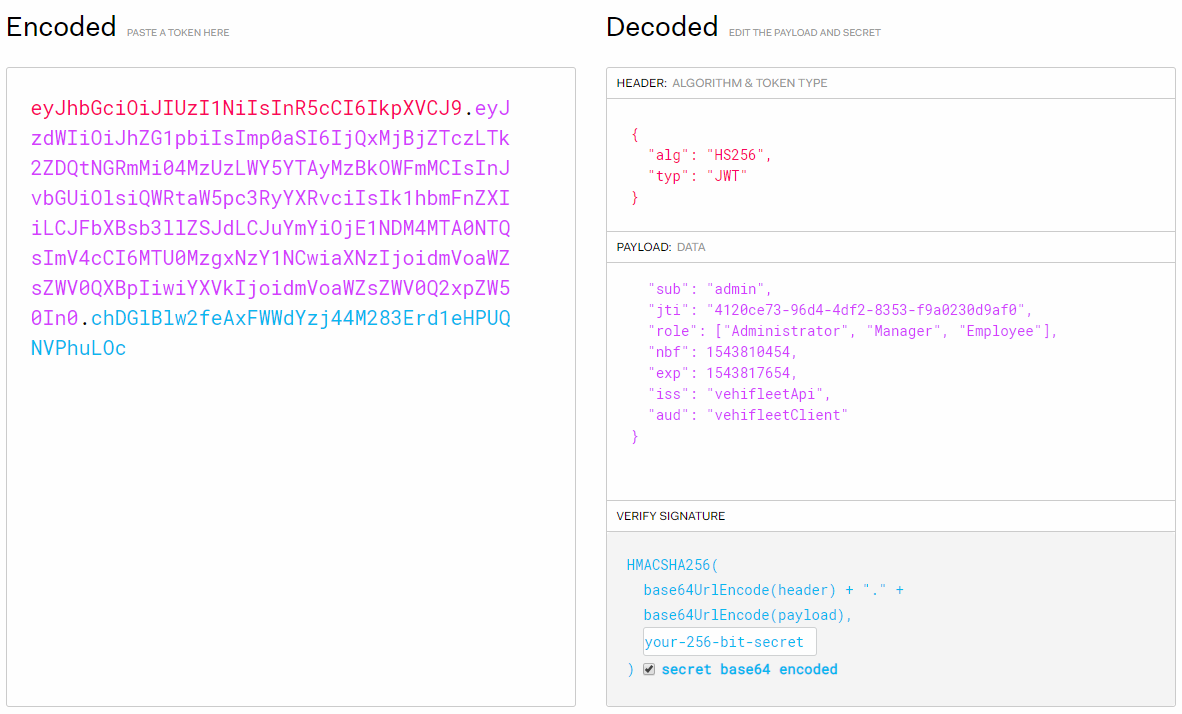
\includegraphics[scale=0.54]{images/jwt.png}
	\caption{Przykładowy token \textit{JWT}}
	\small 
	Token został wygenerowany przy użyciu narzędzia ze strony \textit{https://jwt.io/}.
\end{figure}
\section{Konteneryzacja}
%----------------------------------------------------------------------------------------
%	SECTION 6
%----------------------------------------------------------------------------------------
\newpage
\chapter{Implementacja}

%----------------------------------------------------------------------------------------
%	SECTION 7
%----------------------------------------------------------------------------------------
\newpage
\chapter{Testy}

%----------------------------------------------------------------------------------------
%	SECTION 8
%----------------------------------------------------------------------------------------
\newpage
\chapter{Podsumowanie}
\section{Wnioski}
\section{Możliwości rozwoju}

%----------------------------------------------------------------------------------------
%	SECTION OLD
%----------------------------------------------------------------------------------------

%\chapter{Projekt systemu}
%System można podzielić na dwa elementy — interfejs użytkownika (\textit{UI}) oraz interfejs programistyczny (\textit{API}). Komunikacja między interfejsami odbywa się według protokołu \textit{HTTP}; dane przesyłane są w formacie \textit{JSON}.
%
%Dostęp do systemu został zabezpieczony przy użyciu standardu \textit{JSON Web Token (JWT)}. Autoryzacja \textit{JWT} działa w następujący sposób:
%\begin{enumerate}
%	\item Użytkownik loguje się przez interfejs użytkownika, podając nazwę użytkownika oraz hasło
%	\item Interfejs programistyczny weryfikuje dane logowania
%	\item W przypadku prawidłowego hasła utworzony zostaje token \textit{JWT} zawierający:
%		\subitem Informacje o wydającym token
%		\subitem Informacje o użytkowniku: jego identyfikator (nazwa użytkownika) oraz role
%	\item Utworzony token zostaje zaszyfrowany (uniemożliwiając jego sfałszowanie)i przesłany 		
%	\item Odebrany token zostaje umieszczony w pamięci przeglądarki internetowej użytkownika
%\end{enumerate}
%Interfejs programistyczny weryfikuje poprawność tokena dla każdego żądania \textit{HTTP} z wyjątkiem tych związanych z procesem autoryzacji użytkownika; jeżeli token jest niepoprawny lub zbyt stary (wydany więcej niż 2 godziny przed weryfikacją), żądanie jest odrzucone.
%
%
%[[ tutaj dodam zdjęcie tokenu z systemu przed i po szyfrowaniu ]]

%----------------------------------------------------------------------------------------
%	APPENDIX
%----------------------------------------------------------------------------------------
%\appendix
%\chapter{Donec cursus nulla vitae pede}
%Donec cursus nulla vitae pede. Etiam quam pede, aliquet ut, pellentesque sed, sagittis non, est. Quisque egestas malesuada risus. Maecenas ultricies libero a quam. Nullam feugiat arcu. Class aptent taciti sociosqu ad litora torquent per conubia nostra, per inceptos hymenaeos. In interdum, risus ut gravida sollicitudin, leo sapien commodo dui, non consectetuer nisl nunc ac massa. Mauris a orci in eros venenatis euismod. Curabitur orci. Quisque pharetra, dui sed dignissim hendrerit, nibh ante malesuada eros, sed tincidunt magna lorem a tellus. Aliquam erat volutpat. Aenean pulvinar, metus et mattis dictum, massa lacus semper purus, quis vehicula augue mi et leo. Ut eu ipsum. Sed dictum dapibus nisi. Cras mattis.

%----------------------------------------------------------------------------------------
%	END
%----------------------------------------------------------------------------------------
\addcontentsline{toc}{chapter}{Literatura}
\bibliography{bibliography}

%opcjonalnie może się tu pojawić spis rysunków i tabel
\listoffigures
\listoftables
\end{document}

